При поиске места проведения соревнования --- UQ Центра, вы заблудились и оказались в секретной группе пещер под университетом. Вход в группу пещер преграждает система безопасности, включающая в себя $N$ дверей, расположенных друг за другом, и $N$ переключателей, каждый из которых соединён только с одной из дверей. Различные переключатели соединены с различными дверями.
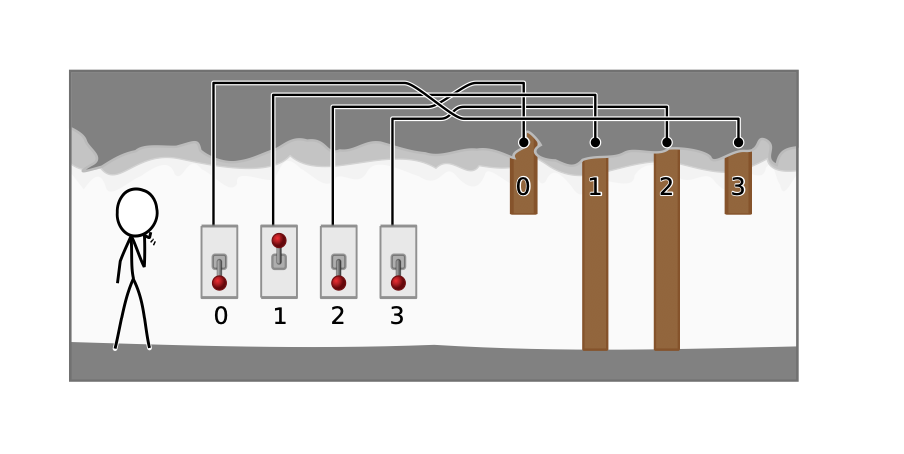
\includegraphics{cave1.png}
Двери пронумерованы от входа в группу пещер от $0$ до $(N - 1)$ в порядке от ближних к дальним. Переключатели также пронумерованы от $0$ до $(N - 1)$, однако, вы не знаете, с какой дверью соединен каждый переключатель.

Все переключатели расположены у входа в группу пещер. Каждый переключатель может быть в одном из двух положений: <<вверх>> или <<вниз>>. Одно из этих положений является правильным. Если он находится в правильном положении, то соединенная с переключателем дверь будет открыта, иначе эта дверь будет закрыта. Правильное положение может различаться для разных переключателей, и вы не знаете, какое из положений для какого переключателя является правильным.

Вы хотите понять, как устроена система безопасности. Для этого вы можете задать комбинацию положений переключателей, то есть установить каждый из переключателей в любое из положений; после чего войти в пещеру и узнать номер первой закрытой двери. Двери, находящиеся за ней, не видны.

У вас есть время на то, чтобы попробовать не более $70\,000$ комбинаций положений переключателей. Ваша задача --- определить правильное положение для каждого переключателя, а также для каждого переключателя найти дверь, с которой он соединен.

Ваше решение должно реализовывать функцию \t{exploreCave()}. Она может вызывать функцию проверяющего модуля \t{tryCombination()} не более $70\,000$ раз и должна завершаться вызовом функции \t{answer()}. Эти функции описаны ниже.

Функция проверяющего модуля \t{tryCombination()}:

\t{int tryCombination(int S[]);}

Эту функцию реализует проверяющий модуль. Она позволяет вам задать комбинацию положений переключателей для того, чтобы войти в группу пещер и узнать номер первой закрытой двери. Если все двери открыты, то функция возвращает значение
­$-1$. Эта функция работает за время $O(N)$ , то есть время работы в худшем случае пропорционально $N$.

Эта функция может быть вызвана не более $70\,000$ раз.

Параметры:
\begin{itemize}
\item $S$: массив длины $N$, задающий комбинацию положений переключателей. Элемент массива $S[i]$ соответствует переключателю с номером $i$. Значение $0$ означает, что переключатель находится в положении <<вверх>>. Значение $1$ означает, что переключатель находится в положении <<вниз>>.
\item \textit{Возвращаемое значение}: номер первой закрытой двери или $­-1$, если все двери открыты.
\end{itemize}



Функция проверяющего модуля \t{answer()}:

\t{void answer(int S[], int D[]);}

Вызовите эту функцию, когда определена комбинация положений переключателей, при которой все двери открыты, а также для каждого переключателя определена дверь, с которой он соединён.

Параметры:
\begin{itemize}
\item $S$: массив длины $N$, содержащий правильное положение каждого переключателя. Формат данного массива такой же, как и у параметра вышеописанной функции \t{tryCombination()}.
\item $D$: массив длины $N$, элементы которого для каждого переключателя задают, с какой дверью он соединён. Элемент $D[i]$ должен содержать номер двери, с которой соединён переключатель с номером $i$.
\item \textit{Возвращаемое значение}: эта функция не возвращает управление вашей программе, то есть приводит к завершению вашей программы.
\end{itemize}



Ваша функция \t{exploreCave()}:

\t{void exploreCave(int N);}

Ваше решение должно реализовывать эту функцию.

Эта функция должна использовать функцию проверяющего модуля \t{tryCombination()}, чтобы определить правильное положение для каждого переключателя, а также для каждого переключателя определить дверь, с которой он соединен. Когда ваша функция получит эту информацию, она должна вызвать
функцию \t{answer()}.

Параметры:
\begin{itemize}
\item $N$: количество переключателей и дверей в группе пещер.
\end{itemize}
